%%%%%%%%%%%%%%%%%%%%%%%%%%%%%%%%%%%%%%%%%%%%%%%%%%%%%%%%%%%%%%%%%%%%%%%%%%%%%%%%
% CSC2059 Practical 10
%%%%%%%%%%%%%%%%%%%%%%%%%%%%%%%%%%%%%%%%%%%%%%%%%%%%%%%%%%%%%%%%%%%%%%%%%%%%%%%%

\documentclass{csc2059practical}

% Additional packages used by this practical.
% TikZ will be used during the visual design pass.
\usepackage{tikz}
\usetikzlibrary{arrows.meta, positioning, fit, backgrounds}
\usepackage{fontawesome5}
\usepackage{booktabs}


\setpracticalnumber{10}

\setpracticaltitle{Choosing the Right Tool}

\setpracticalsubtitle{Searching and Sorting}

\setpracticalauthor{
Dr Giuseppe Trombino\\
School of Electronics, Electrical Engineering and Computer Science\\
Queen's University Belfast
}
\setpracticaldate{}

\usetikzlibrary{arrows.meta,positioning,calc}



\begin{document}

\maketitle

\tableofcontents
\clearpage
%%%%%%%%%%%%%%%%%%%%%%%%%%%%%%%%%%%%%%%%%%%%%%%%%%%%%%%%%%%%%%%%%%%%%%%%%%%%%%%%
\frontsection{Introduction}

Throughout this module you have implemented a variety of data structures and algorithms, each designed to solve a particular problem efficiently. From dynamic arrays and linked lists to binary search trees, every solution has offered different strengths and trade-offs.

In professional software development, however, engineers rarely ask \emph{"What is the best algorithm?"} Instead, they ask \emph{"Which algorithm is best suited to this problem?"}

In this practical you will continue developing the university library catalogue. Librarians need to locate individual books almost instantly when given a catalogue number, while also producing alphabetical catalogues for visitors. Although both tasks involve the same collection of books, they require very different approaches.

By the end of this practical you will have implemented, measured and compared several algorithms before using experimental evidence to justify your engineering decisions.

\begin{learningoutcomes}
By the end of this practical you should be able to:

\begin{itemize}
    \item Explain how hash tables provide efficient lookup using a hash function.
    \item Implement key operations within a hash table.
    \item Export data from one data structure into another representation.
    \item Implement and compare different sorting algorithms.
    \item Use instrumentation to measure the work performed by an algorithm.
    \item Evaluate the suitability of different algorithms for different requirements.
    \item Justify algorithmic choices using experimental evidence.
\end{itemize}
\end{learningoutcomes}

\begin{engineeringquestion}
Can a single data structure provide the best solution for every software engineering problem, or do different requirements demand different approaches?
\end{engineeringquestion}

\begin{infobox}{Estimated Completion Time}

This practical is designed to be completed in approximately \textbf{2 hours}.

\begin{center}
\begin{tabular}{lr}
\toprule
Activity & Approximate Time \\
\midrule
Before You Begin & 10 minutes \\
Part A -- Fast Book Lookup with Hash Tables & 25 minutes \\
Part B -- Exploring the Catalogue & 15 minutes \\
Part C -- Building an Alphabetical Catalogue & 35 minutes \\
Part D -- Choosing a Better Sorting Algorithm & 30 minutes \\
Reflection and Challenge & 5 minutes \\
\bottomrule
\end{tabular}
\end{center}

\end{infobox}

%%%%%%%%%%%%%%%%%%%%%%%%%%%%%%%%%%%%%%%%%%%%%%%%%%%%%%%%%%%%%%%%%%%%%%%%%%%%%%%%
\frontsection{Before You Begin}

Before starting this practical, you should be comfortable with the workflow developed throughout this module. In particular, you should be able to:

\begin{itemize}
    \item Open your GitHub Classroom repository in Visual Studio Code.
    \item Build the supplied code using the provided Makefile.
    \item Run the supplied examples and automated Catch2 tests.
    \item Read and interpret test failures.
    \item Commit and push your work to GitHub regularly.
\end{itemize}

If any of these tasks are unfamiliar, revisit the earlier practicals before continuing.

%%%%%%%%%%%%%%%%%%%%%%%%%%%%%%%%%%%%%%%%%%%%%%%%%%%%%%%%%%%%%%%%%%%%%%%%%%%%%%%%
\frontsection{Important Background Information}

Throughout this module you have explored several different data structures and algorithms. Each was designed to perform certain operations efficiently while making compromises elsewhere.

For example, linked lists make insertion and deletion straightforward but are slower to search than arrays. Binary search trees support efficient searching when organised correctly, while arrays are often better suited to sequential processing.

There is rarely a single \emph{best} solution to every problem. Instead, software engineers evaluate the requirements of an application before selecting the data structures and algorithms that best support those requirements.

In this practical you will compare several approaches to storing, searching and organising the same collection of books. Rather than relying on intuition, you will measure the work performed by each algorithm and use the results to evaluate their suitability.

%%%%%%%%%%%%%%%%%%%%%%%%%%%%%%%%%%%%%%%%%%%%%%%%%%%%%%%%%%%%%%%%%%%%%%%%%%%%%%%%
\frontsection{Getting to Know the Repository}

As with previous practicals, the repository already contains the project structure, automated tests and demonstration programs required to complete the exercises.

The repository is organised as follows:

\begin{center}
\begin{tabular}{ll}
\toprule
Folder & Description \\
\midrule
\texttt{include/} & Header files for the supplied classes and interfaces. \\
\texttt{src/} & Source files containing the implementations you will complete. \\
\texttt{tests/} & Automated Catch2 test suites. \\
\texttt{examples/} & Demonstration programs used throughout the practical. \\
\texttt{data/} & Sample datasets used by the library catalogue. \\
\bottomrule
\end{tabular}
\end{center}

The practical follows the same Test-Driven Development workflow used throughout this module.

\begin{itemize}
    \item Complete the tasks for each part.
    \item Run the corresponding test suite.
    \item Fix any failing tests.
    \item Run the demonstration program.
    \item Commit your work before moving to the next part.
\end{itemize}

The following commands will be used throughout the practical:

\begin{terminal}
make test01
make example01

make example02

make test02
make example03

make test03
make example04
\end{terminal}

You can also execute every test suite or every demonstration program using:

\begin{terminal}
make test
make run
\end{terminal}

\section{Part A -- Faster Searches with Hash Tables}
\begin{infobox}[Estimated time]
    This section should take approx 30 minutes to complete
\end{infobox}

\subsection*{Engineering Problem}

In Practical 8, you investigated different ways of searching for books in a library catalogue. Although some approaches performed better than others, they all shared one important characteristic: the search algorithm still needed to examine existing records until the required book was found. As the catalogue grows, the amount of work required also increases.

Software engineers often solve problems by looking beyond the algorithm itself. Instead of asking:

\begin{quote}
\emph{Can we write a faster search algorithm?}
\end{quote}

they ask a different question:

\begin{quote}
\emph{Can we organise the data differently so that finding a book becomes much easier?}
\end{quote}

One common solution is a \textbf{hash table}. Rather than storing books sequentially, a hash table uses each book's unique catalogue number to calculate where it should be stored. When searching for a book, the same calculation is performed again, allowing the software to jump directly to the correct location instead of examining every record one by one.

\begin{figure}[htbp]
    \centering
    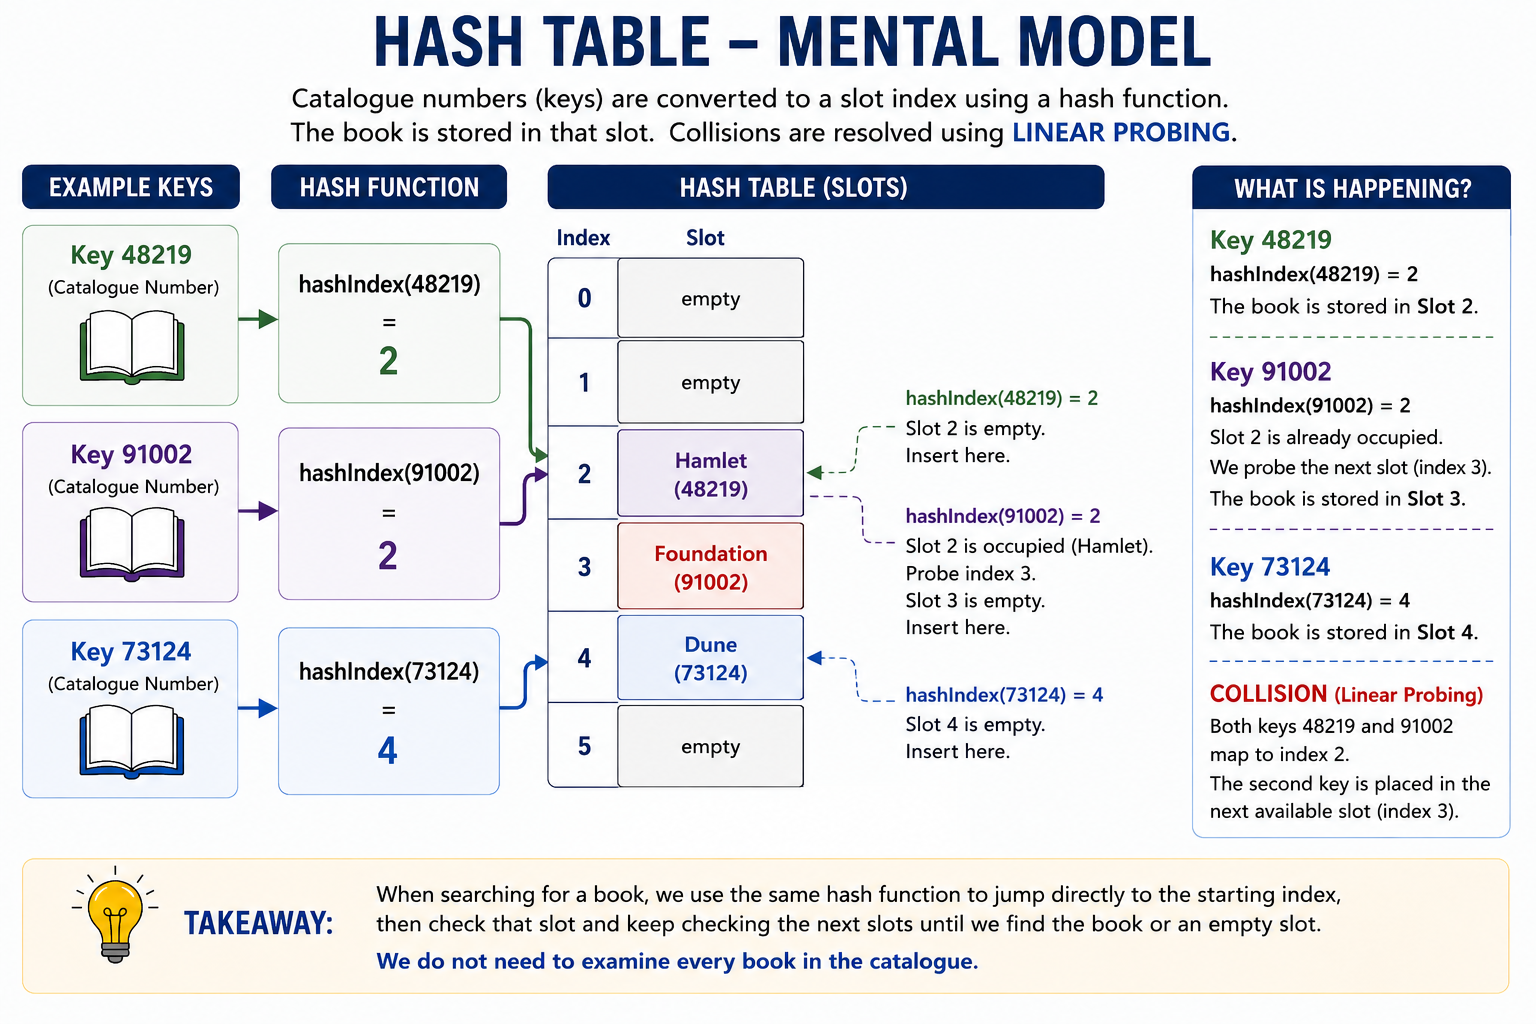
\includegraphics[
        width=\textwidth,
        height=0.4\textheight,
        keepaspectratio
    ]{../../../assets/figures/practical10/hash_table_new.png}
    \caption{Mental model of a hash table, showing how catalogue numbers are mapped to buckets and how collisions are handled using probing.}
    \label{fig:hash-table-mental-model}
\end{figure}

In this part of the practical, you will complete the missing components of a simple hash table and observe how reorganising the data can reduce the amount of work required to perform a search.

\begin{importantnote}
Notice that we have not changed the search problem itself. Instead, we have changed \emph{how the data is organised}. This is an important distinction that software engineers make when designing efficient systems.
\end{importantnote}

\subsection*{Run the Demonstration}

Compile and run the first example program:

\begin{terminal}
make example01
\end{terminal}

The demonstration loads the library catalogue into a hash table and attempts to search for three books.

At the moment, however, none of the searches succeed because two important functions have been left incomplete. Before making any changes, run the program and observe its current behaviour.

\subsection*{Your Tasks}

Open \texttt{HashTable.cpp} and complete the following functions:

\begin{enumerate}
    \item \texttt{hashIndex()}\\
    Implement the hash function that converts a catalogue number into the appropriate bucket within the hash table.

    \item \texttt{find()}\\
    Use the calculated bucket index to locate and return the requested book from the appropriate bucket.
\end{enumerate}

As you complete each function, run the public tests regularly to verify your progress.

\begin{terminal}
make test01
\end{terminal}

Once all of the tests pass, run the demonstration again to confirm that all three searches now return the correct books.

\clearpage

\begin{reflectionbox}
Have we improved the search algorithm itself, or have we solved the problem by organising the data differently?

Why might this approach become increasingly attractive as the library catalogue continues to grow?
\end{reflectionbox}

\section{Part B -- When Requirements Change}
\begin{infobox}[Estimated time]
    You should spend no more than 10 minutes in this section
\end{infobox}

\subsection{Requirement Creep}

The new catalogue system has been a success. Visitors can now locate books quickly using their catalogue numbers, and the library staff are pleased with the improvement.

A few weeks later, however, a new request arrives:

\begin{quote}
\emph{"Could we also print an alphabetical list of every book in the catalogue for visitors to browse?"}
\end{quote}

At first glance, this seems like a small change. After all, the books are already stored in the system.

\begin{tipbox}
Software projects rarely remain unchanged. As users begin using a system, new ideas and additional features are often requested. This gradual expansion of a system's original goals is commonly known as requirement creep.
\end{tipbox}

Compile and run the second example program:

\begin{terminal}
make example02
\end{terminal}

The example prints every book stored in the hash table.

Unfortunately, the output is not arranged alphabetically. Instead, the books appear grouped according to the buckets in which they were stored, making the catalogue difficult for visitors to browse.

\begin{importantnote}
This is not a fault in the hash table. The hash table is behaving exactly as intended---it organises books for \emph{fast retrieval by catalogue number}, not for maintaining alphabetical order.
\end{importantnote}

Software engineering often involves balancing competing requirements. A solution that is ideal for one task may be unsuitable for another.

In this case, we have discovered that fast searching alone is no longer sufficient. If we want to present books in alphabetical order, we first need a way to rearrange the data.

This process is known as \textbf{sorting}.

\begin{reflectionbox}
Why can't a hash table easily produce an alphabetical catalogue?

What information determines where a book is stored inside the hash table, and why does this conflict with alphabetical ordering?
\end{reflectionbox}

\section{Part C -- Restoring Order with Bubble Sort}
\begin{infobox}[Estimated Time]
    This section should take approximately 35 minutes to complete.
\end{infobox}

\subsection{Sorting the Catalogue}

The hash table has successfully solved the problem of finding individual books quickly, but it cannot produce an alphabetical catalogue.

To meet the library's new requirement, the books must first be arranged into the correct order.

This process is called \textbf{sorting}. A sorting algorithm repeatedly compares items and rearranges them until they appear in the required sequence.

In this part of the practical, you will implement one of the simplest sorting algorithms: \textbf{Bubble Sort}. Although Bubble Sort is not the most efficient sorting algorithm, it is easy to understand and provides an excellent introduction to the ideas behind sorting.

\begin{figure}[htbp]
    \centering
    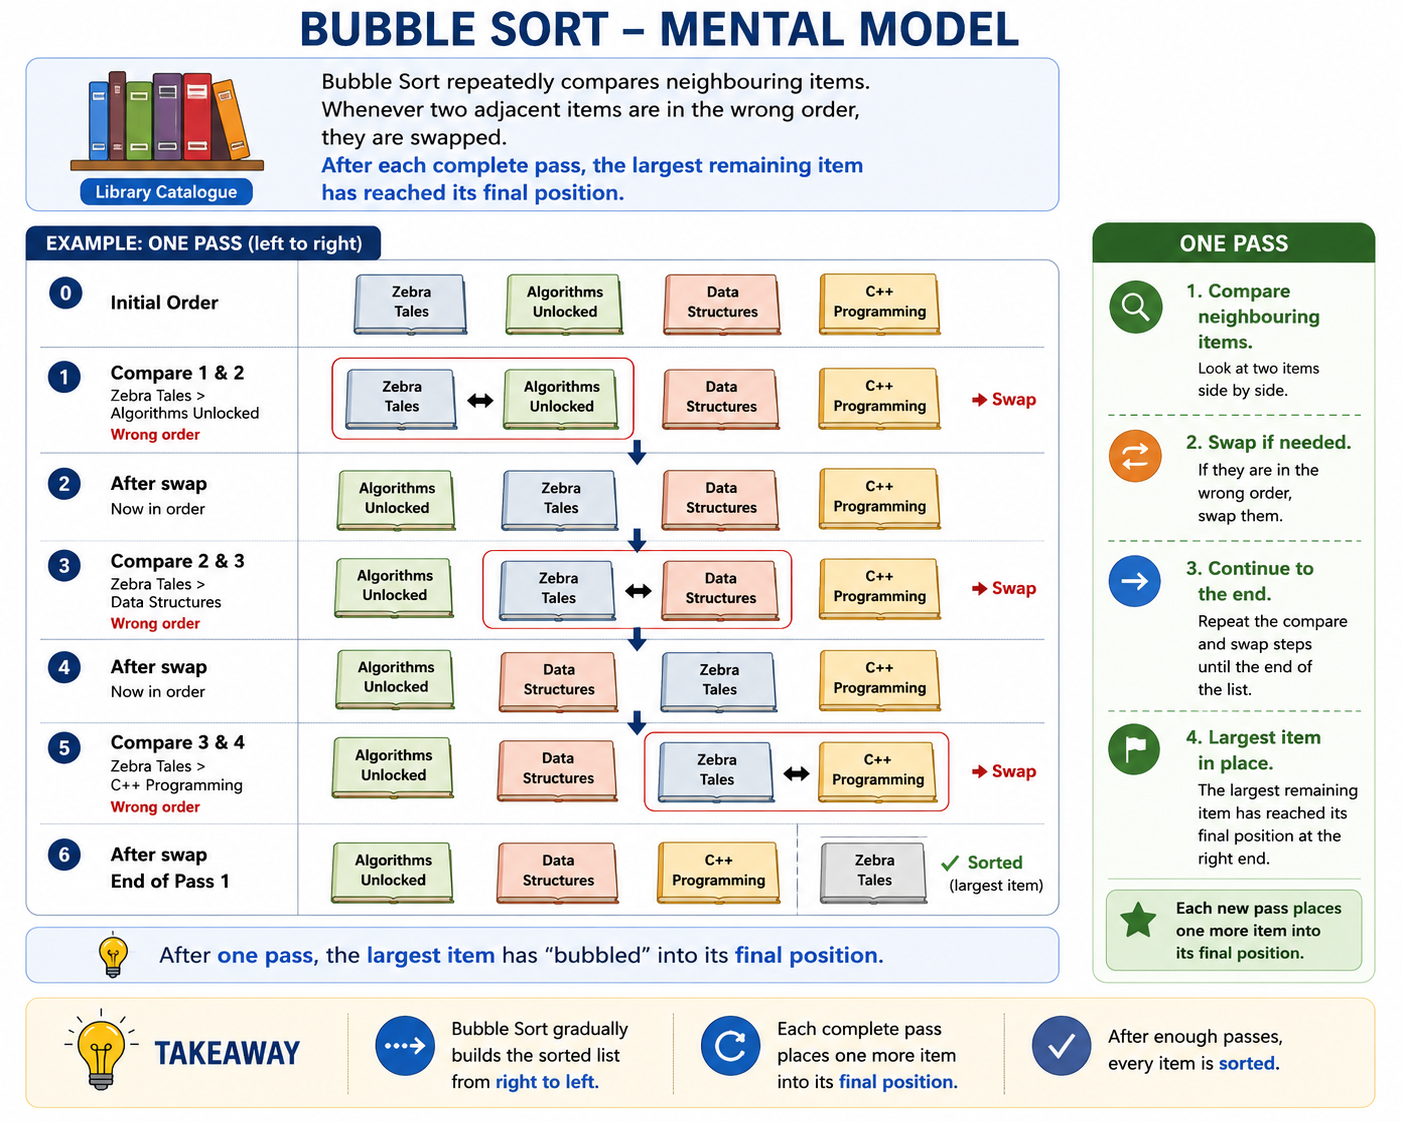
\includegraphics[
        width=\textwidth,
        height=0.4\textheight,
        keepaspectratio
    ]{../../../assets/figures/practical10/bubble_sort.png}
    \caption{One complete pass of Bubble Sort. Neighbouring books are compared and swapped until the largest remaining item reaches its final position.}

    \label{fig:bubble-sort-mental-model}

\end{figure}


\subsection{Run the Demonstration}

Compile and run the third example program:

\begin{terminal}
make example03
\end{terminal}

The example loads the canonical library dataset and attempts to print the books in alphabetical order.

At the moment, however, the output remains unsorted because the Bubble Sort algorithm has not yet been implemented.

\subsection{Your Tasks}

Open \texttt{Sorting.cpp} and complete the implementation of the \texttt{bubbleSortByTitle()} function and the helper functions \texttt{comesBefore()} and \texttt{swapBooks()}.

As you develop your solution, run the public tests regularly to verify your progress.

\begin{terminal}
make test02
\end{terminal}

Once all of the tests pass, run the demonstration again and confirm that the catalogue is now printed in alphabetical order.

\begin{tipbox}
Bubble Sort repeatedly compares neighbouring books and swaps them whenever they appear in the wrong order. After each complete pass through the data, one more book reaches its correct position in the sorted catalogue.
\end{tipbox}

\begin{reflectionbox}
Bubble Sort solves the library's new requirement, but how much work does it perform to sort a large collection of books?

Would the same approach still be appropriate if the catalogue contained tens of thousands of records?
\end{reflectionbox}

\section{Part D -- Scaling Up with Quick Sort}
\begin{infobox}[Estimated time]
    This section should take approximately 40 minutes to complete.
\end{infobox}

\subsection{When the Catalogue Keeps Growing}

Bubble Sort has successfully solved the library's new requirement. The books can now be arranged alphabetically, making the catalogue much easier for visitors to browse.

Unfortunately, the story does not end there.

Over the next few years, the library continues to expand. Thousands of new books are added to the catalogue, which now contains more than 10,000 records.

Although Bubble Sort still produces the correct result, the staff begin to notice that generating an alphabetical catalogue takes much longer than before.

The algorithm is correct, but it is no longer the most appropriate solution for a catalogue of this size.

Software engineers regularly encounter situations like this. As systems grow, algorithms that were perfectly acceptable for small datasets may become impractical. Rather than changing the requirement, they look for a more efficient algorithm that solves the same problem.

One such algorithm is \textbf{Quick Sort}.

\begin{figure}[htbp]
    \centering
    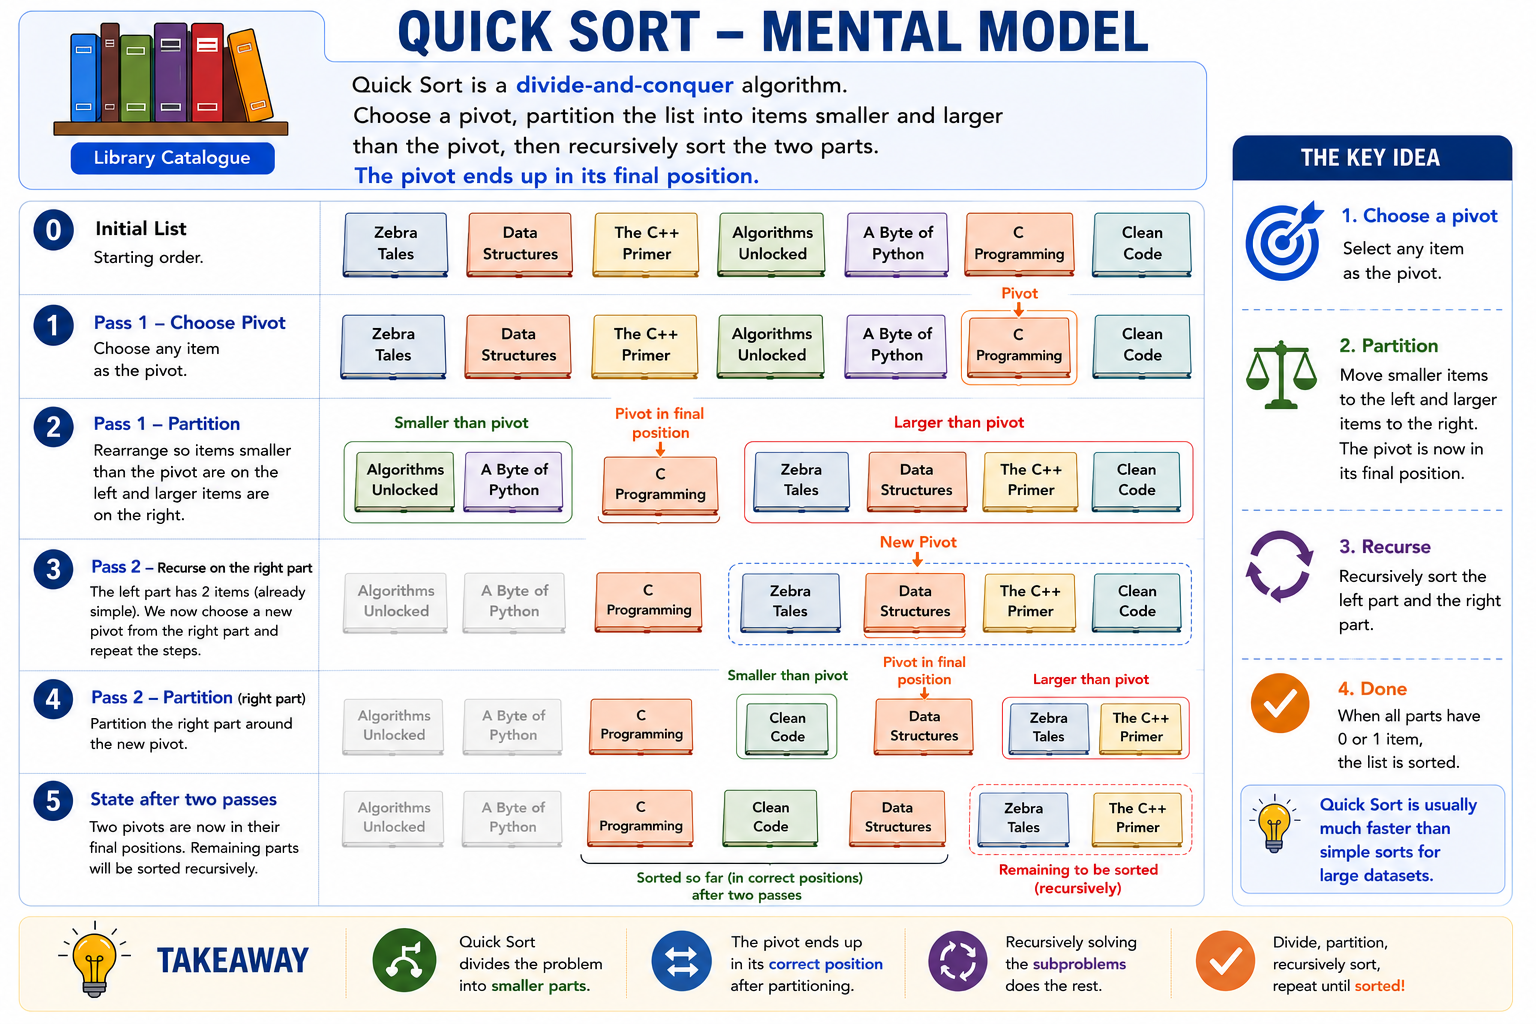
\includegraphics[
        width=\textwidth,
        height=0.4\textheight,
        keepaspectratio
    ]{../../../assets/figures/practical10/quick_sort.png}
    \caption{Mental model of Quick Sort, showing pivot selection, partitioning, and the recursive processing of smaller subproblems.  Note: the left side of the figure (greyed out) has not been sorted yet}

    \label{fig:quick-sort-mental-model}

\end{figure}

\subsection{Run the Demonstration}

Compile and run the fourth example program:

\begin{terminal}
make example04
\end{terminal}

The demonstration loads the larger application dataset and compares the work performed by Bubble Sort and Quick Sort.

At the moment, Quick Sort has not yet been implemented, so the comparison cannot be completed.

\subsection*{Your Tasks}

Open \texttt{Sorting.cpp} and complete the implementation of the following functions:

\begin{itemize}
    \item \texttt{partition()}
    \item \texttt{quickSortByTitle()}
\end{itemize}

As before, run the public tests regularly while developing your solution.

\begin{terminal}
make test03
\end{terminal}

Once all of the tests pass, run the demonstration again and compare the amount of work performed by each sorting algorithm.

\begin{importantnote}
Both algorithms produce exactly the same alphabetical catalogue.

The difference lies not in the correctness of the result, but in the amount of work required to produce it.
\end{importantnote}

\begin{reflectionbox}
Bubble Sort and Quick Sort solve exactly the same problem.

Why would a software engineer choose one algorithm over the other?

How does the size of the dataset influence that decision?
\end{reflectionbox}

\section{Part E -- Choosing the Right Tool}
\begin{infobox}[Estimated time]
    Please take at least 20 minutes completing this section (can be done out of the lab).
\end{infobox}

Throughout this module, you have implemented and explored a wide range of data structures and algorithms.

You have seen that each solution has strengths, weaknesses, and assumptions. A structure designed for fast searching may not preserve order. An algorithm that performs well on a small dataset may become unsuitable as the dataset grows.

Software engineers therefore rarely ask:

\begin{quote}
\emph{Which data structure or algorithm is the best?}
\end{quote}

Instead, they ask:

\begin{quote}
\emph{Which data structure or algorithm is the most appropriate for this particular problem?}
\end{quote}

For each of the following real-world scenarios:

\begin{enumerate}
    \item recommend an appropriate data structure;
    \item identify an appropriate algorithm or operation, where relevant;
    \item briefly justify your decision.
\end{enumerate}

There may be more than one reasonable answer. Your justification is more important than selecting one particular structure.

\subsection*{Scenario 1 -- Emergency Department Queue}

Patients arrive at an emergency department and wait to be assessed. In most cases, patients should be processed in the order in which they arrive.

However, critically ill patients may need to be treated before patients who arrived earlier.

\begin{reflectionbox}
Which data structure would you use to organise the patients?

Would a normal queue be sufficient, or would the system need additional information to determine who should be treated next?
\end{reflectionbox}

\subsection*{Scenario 2 -- Browser History}

A web browser records each page visited by the user.

The user should be able to move backwards through previously visited pages and then move forwards again if they have not opened a new page.

\begin{reflectionbox}
Which data structure or combination of data structures would support the Back and Forward buttons?

Which operations would be performed when the user visits a new page?
\end{reflectionbox}

\subsection*{Scenario 3 -- University Student Records}

A university stores records for thousands of students.

Staff frequently need to retrieve a student using their unique student number. They may also occasionally need to produce an alphabetically ordered class list.

\begin{reflectionbox}
Which data structure would you use for fast retrieval by student number?

Would the same structure be ideal for producing the alphabetical list? Explain any trade-offs involved.
\end{reflectionbox}

\subsection*{Scenario 4 -- GPS Route Planning}

A navigation system stores roads connecting towns and cities.

Each road has an associated distance or estimated travel time. The system must calculate a route between two locations.

\begin{reflectionbox}
Which data structure would you use to represent the road network?

Which type of algorithm would be required to find an appropriate route?
\end{reflectionbox}

\subsection*{Scenario 5 -- Undo and Redo}

A drawing application records each action performed by the user.

Selecting Undo should reverse the most recent action. Selecting Redo should restore an action that has just been undone.

\begin{reflectionbox}
Which data structure or combination of data structures would support Undo and Redo?

Why is the order in which actions are removed important?
\end{reflectionbox}

\subsection*{Scenario 6 -- Music Playlist}

A music application allows users to:

\begin{itemize}
    \item play songs in sequence;
    \item insert a new song anywhere in a playlist;
    \item remove songs;
    \item move forwards and backwards through the playlist.
\end{itemize}

\begin{reflectionbox}
Which data structure would you use to represent the playlist?

Would an array or a linked structure be more appropriate? What operations influence your decision?
\end{reflectionbox}

\subsection*{Scenario 7 -- Dictionary and Spell Checker}

A spell checker stores a large collection of valid words.

For every word typed by the user, the software must quickly determine whether that word exists in the dictionary.

\begin{reflectionbox}
Which data structure would support fast membership checks?

What information could be used to determine where each word is stored?
\end{reflectionbox}

\subsection*{Scenario 8 -- Organisation Chart}

A company is organised into departments, teams, and individual employees.

Each employee normally reports to one manager, while each manager may supervise several employees.

\begin{reflectionbox}
Which data structure would represent this hierarchy?

Which traversal could be used to print everyone working beneath a particular manager?
\end{reflectionbox}

\subsection*{Scenario 9 -- Social Network}

A social networking platform stores millions of users and the connections between them.

The system must support tasks such as:

\begin{itemize}
    \item identifying whether two users are connected;
    \item finding mutual connections;
    \item suggesting a chain of connections between two users.
\end{itemize}

\begin{reflectionbox}
Which data structure would you use to represent users and their connections?

Which algorithms or traversals could help answer these questions?
\end{reflectionbox}

\subsection*{Scenario 10 -- Online Shop Catalogue}

An online shop stores thousands of products.

Customers may:

\begin{itemize}
    \item search for a product using its unique product code;
    \item browse products alphabetically;
    \item sort products by price;
    \item display only products belonging to a particular category.
\end{itemize}

\begin{reflectionbox}
Would one data structure efficiently support every requirement?

Which structures and algorithms might be combined to support the different operations?
\end{reflectionbox}

\clearpage

\begin{figure}[p]
    \centering
    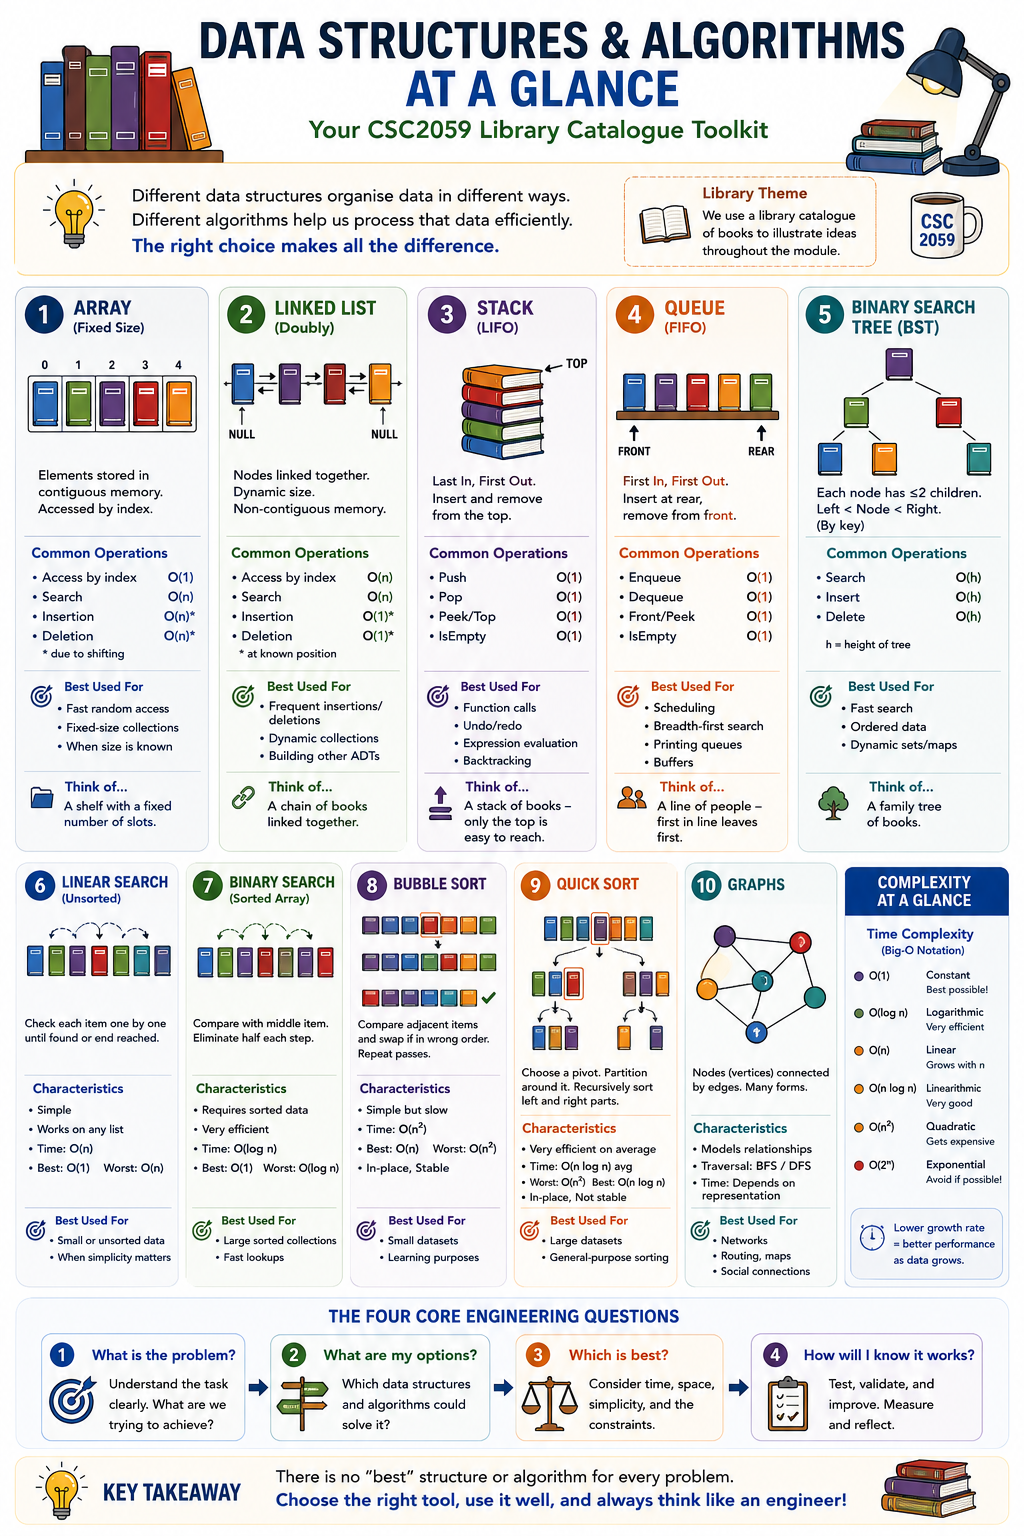
\includegraphics[
        width=\textwidth,
        height=0.92\textheight,
        keepaspectratio
    ]{../../../assets/figures/practical10/summary.png}
    \caption{DSA At a glance}
    \label{fig:dsa-at-a-glance}
\end{figure}

\clearpage


\begin{wrapupbox}


Throughout CSC2059, you have worked with arrays, linked lists, stacks, queues, trees, graphs, hash tables, searching algorithms, and sorting algorithms.

None of these solutions is universally best.

A good software engineer considers:

\begin{itemize}
    \item what operations the system must perform;
    \item how frequently those operations occur;
    \item how much data must be processed;
    \item whether the data must remain ordered;
    \item how the requirements may change in the future.
\end{itemize}

The most important skill is not memorising one preferred solution. It is being able to evaluate the problem, recognise the available trade-offs, and select an appropriate data structure and algorithm.

Congratulations on completing the CSC2059 practical programme.

\end{wrapupbox}

\end{document}
